\documentclass[10pt,onecolumn,twoside,letterpaper]{article}
\usepackage[text={7in,9.5in},centering]{geometry}
\usepackage[spanish,es-nodecimaldot]{babel}

\usepackage{hyperref}

\usepackage{multicol}

\usepackage{harvard}% bibliographystyle: apsr, agsm, dcu, kluwer, nederlands

\usepackage{graphicx}
\usepackage{amssymb}
\usepackage{fancyhdr}
\usepackage{color}
\usepackage{colortbl}
\definecolor{gray}{cmyk}{0.0,0.0,0.0,0.60}

%\usepackage{auto-pst-pdf}
%\usepackage{pst-all}

%\usepackage[numbered]{mcode}
%\usepackage{lipsum}

\pagestyle{fancy}
\fancyhf{}
\fancyhead[RO]{\small{\textcolor{gray}{\textsc{Hacia un framework de locomoci\'on b\'ipeda evolutiva y flexible}}}}
\fancyhead[LO]{
\includegraphics[scale=0.05]{../../images/unlogo.png}}
\fancyhead[LE]{
\includegraphics[scale=0.05]{../../images/unlogo.png}\quad\small{\textcolor{gray}{\textsc{Linea de investigaci\'on: Robotica Evolutiva en Caminadores}}}}
\fancyfoot[CO,CE]{\thepage}
\fancyfoot[LO,RE]{\scriptsize{\textcolor{gray}{\emph{Version 0.2}}}}

\title{\vspace{-0.8cm}
\includegraphics[scale=0.12]{../../images/unescudobn.png}\\\vspace{-0.0cm}
  \LARGE \textbf{Modelos din\'amicos de locomoci\'on b\'ipeda}}
\author{J.A. Castillo-Le\'on\thanks{jacastillol@unal.edu.co} \and R.E. Ram\'irez-Heredia\thanks{reramirezh@unal.edu.co}}
\date{}

\begin{document}
\maketitle
\begin{abstract}\small
  Este trabajo esta enfocado a la construcci\'on, caracterizaci\'on de servos de impedancia variable de bajo costo y un ejemplo ensamblado de al menos cuatro servos. Se requiere fundamentos de dise\~no, microcontroladores y control.
\end{abstract}
%\begin{multicols}{2}
\section{Descripci\'on:}
Basados en el Open Hardware de \cite{Catalano2011}, ver la Figura \ref{fig:servo}, implementando las ideas de la modularidad y construcci\'on r\'apida de impresi\'on 3D, se logra un servo \'util para la interaccion de ambientes impredecibles donde los golpes deben ser aprovechados y reutilizados.
\section{Objetivo:}
El objetivo principal es contruir al menos cuatro servos e implementarlos, para probarlos de forma \emph{Compliance} para caracterizar su desempe\~no. Se preferiria que la estructura construida con los cuatro servos fuera sobre un caminador Talon-Cadera de 4 grados de libertad, en el cual se pueda ver su comportamiento al golpeteo con el piso.
%\end{multicols}
\begin{figure}[!ht]
  \centering
  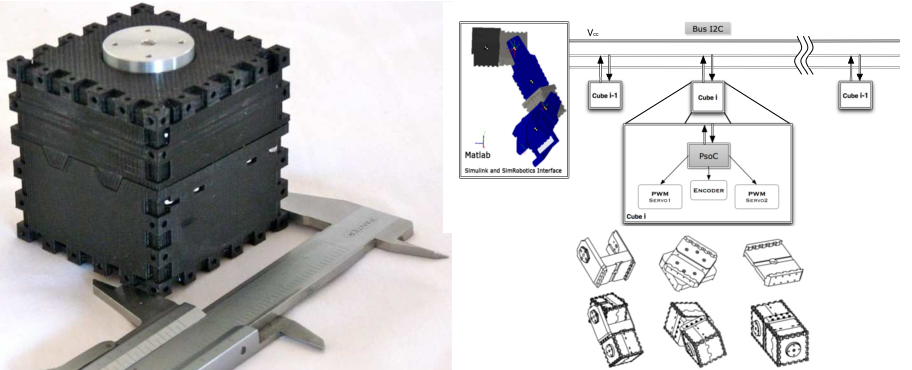
\includegraphics[scale=0.4]{../../images/VSA-CubeBot.png}
  \caption{Modelo Din\'amico General}
  \label{fig:servo}
\end{figure}
%\nocite{*}
\bibliographystyle{nederlands}% apsr, agsm, dcu, kluwer, nederlands
\bibliography{../../review/review/library}
\end{document}
